\chapter{Задача прямой кинематики} \label{ch:2}

\section{Введение} \label{sect2_1}
При разработке манипуляторов(и не только) возникает задача определения положения рабочего элемента по заданным углам. Данная проблема носит название "задача прямой кинематики". Решается с помощью простейших афинных преобразований, которые представляются в виде однородных матриц преобразования координат. Рассмотрим данный метод более подробно.

\section{Однородные координаты и матрицы преобразований}\label{sect2_2}
Имея N-степеней свободы, мы можем представить операцию масштабирования и поворота с помощью матрицы размером $N$x$N$, в то же время мы не можем включить информацию о смещении. На помощь приходят однородные координаты, здесь к обычной матрице поворота добавляется столбец, включающий в себя смещение системы координат.

Например матрица:
\begin{align*}
	\begin{bmatrix}
		1	&	0				&	0				&	dx\\
		0	&	cos(\alpha)		&	-sin(\alpha)	&	dy\\
		0	&	sin(\alpha)		&	cos(\alpha)		&	dz\\
		0	&	0				&	0				&	1
	\end{bmatrix}
\end{align*}
не только поворачивает вектор вокруг оси $x$ на $\alpha$ градусов, но и смещает его на $dx$, $dy$, $dz$ вдоль осей $x$, $y$ и $z$ соответственно.

В качестве примера возьмем манипулятор UR10 фирмы Universal Robotics(см. рис. \ref{fig:ft_sheme1}). 
\begin{figure}[ht]
	\centering
	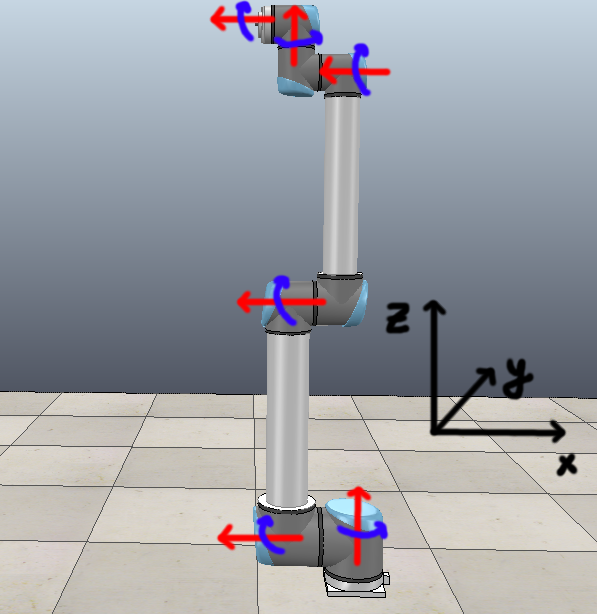
\includegraphics[scale=0.5]{FT/ur10_joints}
	\caption{Схема UR10. Этот рисунок не претендует на звание кинематической схемы. Кинематическую схему см. на рис. \ref{fig:2_2}}
	\label{fig:ft_sheme1}
\end{figure}

На рисунке изображен манипулятор, система координат и направление осей вращения джойнтов. Длины звеньев нам не даны, но имеются абсолютные координаты джойнтов:
\begin{align*}
	O_{0} &= \{0.0000, 0.0000, 0.0000\}\\
	O_{1} &= \{-0.2500, 0.2500, 0.0447\}\\
	O_{2} &= \{-0.3427, 0.2500, 0.1280\}\\
	O_{3} &= \{-0.3621, 0.2506, 0.7401\}\\
	O_{4} &= \{-0.3555, 0.2500, 1.3123\}\\
	O_{5} &= \{-0.4139, 0.2500, 1.3696\}\\
	O_{6} &= \{-0.4712, 0.2500, 1.4282\}\\
	O_{7} &= \{-0.4986, 0.2500, 1.4280\}
\end{align*}

Исходя из данных координат, мы можем найти относительные смещения систем координат:
\begin{align*}
	O_{i, i+1} = O_{i+1} - O_{i}
\end{align*}

Осталось составить сами матрицы переходов между системами координат. Небольшое пояснение к нотации: $\boldsymbol{R_{x/y/z}(q_{i})}$ - матрица поворота вокруг оси $x$, $y$ или $z$ на угол $q_{i}$. $\boldsymbol{\vec{dx}}$ - вектор смещения(первые три элемента четвертого столбца матрицы однородного преобразования). $\boldsymbol{\vec{0}}$ - вектор вида $\{0, 0, 0\}$. С использованием таких определений матрица преобразования принимает вид:
\begin{align*}
	\begin{bmatrix}
		\boldsymbol{R_{axis}(\phi)}		&			\boldsymbol{\vec{dx}}\\
		\boldsymbol{\vec{0}^{T}}		&			1
	\end{bmatrix}
\end{align*}

Матрицы преобразований строятся достаточно шаблонно: нам нужно повернуть вектор вокруг оси вращения джойнта, учитывая направление поворота, и переместить систему координат на вектор относительного смещения повернутый на тот же самый угол вокруг той же самой оси.

Запишем матрицы преобразований:
\begin{align*}
	T_{01} = \begin{bmatrix}
		\boldsymbol{I}					&		\boldsymbol{\vec{O}_{01}}\\
		\boldsymbol{\vec{0}^{T}}		&		1
	\end{bmatrix}
\end{align*}

\begin{align*}
	T_{12} = \begin{bmatrix}
		\boldsymbol{R_{z}(q_{1})}		&		\boldsymbol{R_{z}(q_{1}) \cdot \vec{O}_{12}}\\
		\boldsymbol{\vec{0}^{T}}		&		1
	\end{bmatrix}
\end{align*}

\begin{align*}
	T_{23} = \begin{bmatrix}
		\boldsymbol{R_{x}(-q_{2})}		&		\boldsymbol{R_{x}(-q_{2}) \cdot \vec{O}_{23}}\\
		\boldsymbol{\vec{0}^{T}}		&		1
	\end{bmatrix}
\end{align*}

\begin{align*}
	T_{34} = \begin{bmatrix}
		\boldsymbol{R_{x}(-q_{3})}		&		\boldsymbol{R_{x}(-q_{3}) \cdot \vec{O}_{34}}\\
		\boldsymbol{\vec{0}^{T}}		&		1
	\end{bmatrix}
\end{align*}

\begin{align*}
	T_{45} = \begin{bmatrix}
		\boldsymbol{R_{x}(-q_{4})}		&		\boldsymbol{R_{x}(-q_{4}) \cdot \vec{O}_{45}}\\
		\boldsymbol{\vec{0}^{T}}		&		1
	\end{bmatrix}
\end{align*}

\begin{align*}
	T_{56} = \begin{bmatrix}
		\boldsymbol{R_{z}(q_{5})}		&		\boldsymbol{R_{z}(q_{5}) \cdot \vec{O}_{56}}\\
		\boldsymbol{\vec{0}^{T}}		&		1
	\end{bmatrix}
\end{align*}

\begin{align*}
	T_{67} = \begin{bmatrix}
		\boldsymbol{R_{x}(-q_{6})}		&		\boldsymbol{R_{x}(-q_{6}) \cdot \vec{O}_{67}}\\
		\boldsymbol{\vec{0}^{T}}		&		1
	\end{bmatrix}
\end{align*}

\bigbreak
Полная матрица преобразования:
\begin{align*}
	T = \prod_{i=0}^{6}T_{i,i+1}
\end{align*}

\section{Denavit–Hartenberg conventions и D-H параметры}\label{sect2_3}
В 1955 года Жак Денавит и Ричард Хартенберг разработали соглашение для стандартизации пространственных связей\cite{DenavitHartenberg}. Соглашения очень простые
\begin{itemize}
	\item Координатные системы привязаны к джойнтам
	\item Ось $Z$ координатной системы направлена вдоль оси вращения джойнта.
	\item Ось $X$ параллельна общей нормали осей вращения предыдущего и текущего джойнта $Z_{i-1} \times Z_{i}$.
	\item Ось $Y$ выбирается исходя из $X$ и $Z$ так, чтобы координатная система соответствовала правилу правой руки.
\end{itemize}
\begin{figure}[h!]
	\centering
	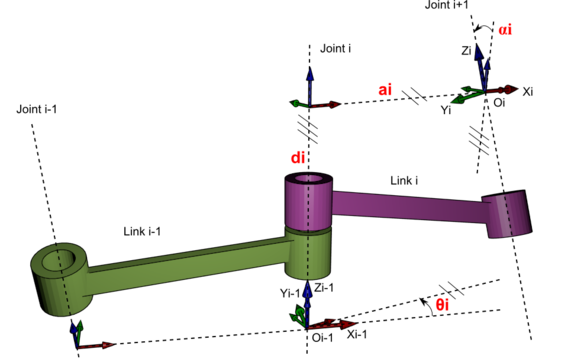
\includegraphics[scale=0.8]{/FT/DHparameters}
	\caption{Пример D-H параметров}
	\label{fig:2_3_1}
\end{figure}
Исходя из вышеуказанных соглашений можно выделить четыре параметра(см. рис. \ref{fig:2_3_1}), необходимых для того, чтобы совершать преобразования:
\begin{itemize}
	\item $d$ - смещение по оси $Z$ предыдущего джойнта до общей нормали. В случае параллельных осей этот параметр выбирается произвольно.
	\item $\theta$ - угол поворота вокруг предыдущего джойнта, необходимый для совмещения осей $X$. Это наш текущий угол поворота джойнта плюс начальное смещение.
	\item $r$ на рисунке обозначен, как $a$ - длина общей нормали.
	\item $\alpha$ - угол поворота вокруг общей нормали, необходимый для совмещения осей $Z$
\end{itemize}
Принимая во внимание указанные выше параметры, можно представить преобразование координат между звеньями как
\begin{align*}
	T = Z_{1}X_{1}T_{2}X_{2} ... Z_{n}X_{n}
\end{align*}
где
\begin{equation}\label{eq:2_3_1}
	\begin{aligned}
		Z_{i} = A_{Z}(d_{i})R_{z}(\theta_{i})\\
		X_{i} = A_{X}(r_{i})R_{x}(\alpha_{i})
	\end{aligned}
\end{equation}
Здесь $A$ - однородна матрица смещения координат, а $R_{a}$ - однородная матрица поворота вокруг оси $a$.

Выполнение данного соглашения усложняет процесс вычисления преобразований, но дает эффективный метод стандартизации и автоматизации расчета прямой кинематики: реализовав алгоритм преобразований в виде \ref{eq:2_3_1} единожды, можно решать задачу прямой кинематики для любого робота, для которого выполняется данное соглашение, не изменяя алгоритма.

Кинематическая схема манипулятора UR10 с учетом вышеописанных соглашений см. на рис. \ref{fig:2_2}, а соответствующие схеме DH параметры на рис. \ref{fig:2_3}.
\begin{figure}[h!]
	\centering
	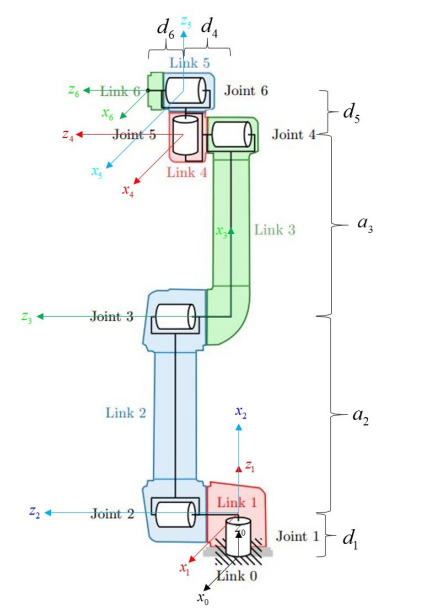
\includegraphics[scale=0.5]{FT/ur10_kinematic_scheme}
	\caption{Кинематическая схема манипулятора UR10.}
	\label{fig:2_2}
\end{figure}
\begin{figure}[h!]
	\centering
	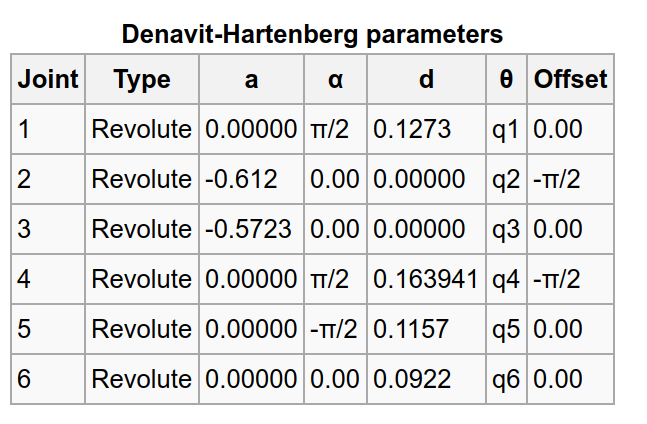
\includegraphics[scale=0.5]{FT/ur10_dh_parameters}
	\caption{DH параметры для манипулятора UR10.}
	\label{fig:2_3}
\end{figure}
